\documentclass[12pt, a4paper, oneside]{ctexbook}
\usepackage{amsmath}
\usepackage{amsfonts}
\usepackage{mathabx}
\usepackage{subcaption} 
\usepackage{cancel}
\usepackage{pifont}
\usepackage{circledsteps}
\usepackage{bm}
\usepackage{tcolorbox}
\usepackage{amsthm,amsmath,amssymb}
\usepackage{floatrow}
\usepackage{caption}
\usepackage{geometry}
\usepackage{graphicx}
\usepackage{wrapfig}
\usepackage{mathtools}
\usepackage{scalerel}    
\usepackage{extarrows}
\usepackage{color,framed,hyperref,mathrsfs}

\title{{\Huge{\textbf{信息论}}}\\——笔记整理}
\author{BarryMafu}
\date{\today}
\linespread{1.5}
\newtheorem{theorem}{定理}[section]
\newtheorem{definition}[theorem]{定义}
\newtheorem{lemma}[theorem]{引理}
\newtheorem{corollary}[theorem]{推论}
\newtheorem{example}[theorem]{例}
\newtheorem{proposition}[theorem]{命题}
\newenvironment{solution}
  {\renewcommand\qedsymbol{$\blacksquare$}\begin{proof}[解答]}
  {\end{proof}}

%----- 自定义命令 -----
\newcommand{\Z}{\mathbb{Z}}
\newcommand{\N}{\mathbb{N}}
\newcommand{\R}{\mathbb{R}}
\newcommand{\Q}{\mathbb{Q}}
\newcommand{\C}{\mathbb{C}}
\newcommand{\E}{\mathbb{E}}
\newcommand{\Pow}{\mathcal{P}}
\newcommand{\cov}{\mathsf{Cov}}
\newcommand{\var}{\mathsf{Var}}
\newcommand{\A}{\mathcal{A}}
\newcommand{\bA}{\boldsymbol{A}}
\newcommand{\ii}{\mathrm{i}\mkern1mu}
\newcommand{\abs}[1]{\left\vert#1\right\vert}
\newcommand{\norm}[1]{\left\lVert#1\right\rVert}
\newcommand{\dx}[1][x]{\mathop{}\!\mathrm{d}#1}
\newcommand{\del}[2]{\dfrac{\partial#1}{\partial#2}}
\newcommand{\red}[1]{\textcolor{red}{#1}}
\newcommand{\emp}[1]{\textcolor[RGB]{193, 0, 53}{#1}}
\newcommand{\sbe}{\ensuremath{\subseteq}}
\newcommand{\spe}{\ensuremath{\supseteq}}
\newcommand{\sbne}{\ensuremath{\subsetneq}}
\newcommand{\spne}{\ensuremath{\supsetneq}}
\newcommand{\Ord}{\ensuremath{\text{Ord}}}
\newcommand{\al}{\ensuremath{\alpha}}
\newcommand{\be}{\ensuremath{\beta}}
\newcommand{\ga}{\ensuremath{\gamma}}
\newcommand{\de}{\ensuremath{\delta}}
\newcommand{\te}{\ensuremath{\theta}}
\newcommand{\et}{\ensuremath{\eta}}
\newcommand{\ld}{\ensuremath{\lambda}}
\newcommand{\Al}{\ensuremath{\bm{\alpha}}}
\newcommand{\Be}{\ensuremath{\bm{\beta}}}
\newcommand{\Ga}{\ensuremath{\bm{\gamma}}}
\newcommand{\De}{\ensuremath{\bm{\delta}}}
\newcommand{\Te}{\ensuremath{\bm{\theta}}}
\newcommand{\Et}{\ensuremath{\bm{\eta}}}
\newcommand{\Xx}{\ensuremath{\bm{\xi}}}
\newcommand{\ci}{\ensuremath{\circ}}
\newcommand{\s}{\ensuremath{\ast}}
\newcommand{\ra}{\ensuremath{\rightarrow}}
\newcommand{\Ra}{\ensuremath{\Rightarrow}}
\newcommand{\la}{\ensuremath{\leftarrow}}
\newcommand{\La}{\ensuremath{\Leftarrow}}
\newcommand{\LR}{\ensuremath{\Leftrightarrow}}
\newcommand{\LLR}{\ensuremath{\Longleftrightarrow}}
\newcommand{\ora}[1]{\overrightarrow{#1}}
\newcommand{\ag}[1]{\langle#1\rangle}
\newcommand{\para}{\mathrel{/\negmedspace/}}
\newcommand{\bPhi}{\boldsymbol{\Phi}}
\newcommand{\bff}{\boldsymbol{f}}
\newcommand{\by}{\boldsymbol{y}}
\newcommand{\bc}{\boldsymbol{c}}
\newcommand{\bxi}{\boldsymbol{\xi}}
\newcommand{\bI}{\boldsymbol{I}}
\newcommand{\bphi}{\boldsymbol{\phi}}
\newcommand{\vvector}[1]{\left(\begin{matrix} #1 \end{matrix}\right)}

\DeclareMathOperator*{\Span}{Span}
\DeclareMathOperator*{\im}{Im}
\DeclareMathOperator*{\rank}{rank}
\DeclareMathOperator*{\card}{card}
\DeclareMathOperator*{\grad}{grad}
\DeclareMathOperator*{\argmax}{argmax}
\DeclareMathOperator*{\epi}{epi}
\DeclareMathOperator*{\maximize}{maximize}
\DeclareMathOperator*{\minimize}{minimize}
\DeclareMathOperator*{\Null}{Null}
\DeclareMathOperator*{\CC}{CC}

\begin{document}

\maketitle

\pagenumbering{roman}
\setcounter{page}{1}

\begin{center}
    \Huge\textbf{前言}
\end{center}~\

临时抱佛脚\~,复习25Spr信息论期末考试用的,比较草率请谅解!

第一版中,将直接采用按照课堂的分割方式。之后第二次整理时再重新划分。

~\\
\begin{flushright}
    \begin{tabular}{c}
        BarryMafu\\
        \today
    \end{tabular}
\end{flushright}

\newpage
\pagenumbering{Roman}
\setcounter{page}{1}
\tableofcontents
\newpage
\setcounter{page}{1}
\pagenumbering{arabic}

\chapter{Lecture 2}

%--- 信息 ----
\begin{center}
    讲师:王立威 \qquad
    课程时间:25.Feb.25th \qquad 
    笔记:25.June.7th
\end{center}

\bigskip

首先,我们不失一般性地考虑如下的通讯需求:
\begin{itemize}
    \item 无限次的通信(infinite communication)
    \item 信息服从某个固定分布(A prob. distribution over the messages)
\end{itemize}

在这样的背景下,我们力求最小化平均编码长度. 

注意到,我们为了接收方可以唯一解码,我们考虑一组无前缀码(Prefix-Free Codes). 值得注意,这只是一个充分条件,而并不是必要条件.  (下面的例子中就可以看出)
\begin{example}
    考虑码字为$\{0, 01\}$,这并不是无前缀的,但可以唯一解码. 
\end{example}

但事实上,考虑可唯一译码,可以归约到考虑无前缀码,这是由如下的定理保证的:
\begin{theorem}
    记$A$表示所有无前缀码,$B$表示所有可唯一译码,显然有$A\sbne B$.  用$l(C,m)$表示使用码$C$编译信息$m$时的码长,那么可以证明 
    \[
    \min_{C\in B} \E_{m \sim P}\Big[l(C,m)\Big] = \min_{C\in A} \E_{m \sim P}\Big[l(C,m)\Big]
    \]
\end{theorem}
\begin{proof}
    此略去. 主要思想是证明对于任意$C^* \in B$使得$\E l(C^*)$达到最小值,都存在一个对应的$\tilde{C}^* \in A$使得$\E l(\tilde{C}^*) = \E l(C^*)$.  
\end{proof} 

有了上面的基础理论,我们来尝试求无前缀码的最短平均码长。 首先,Kraft不等式为我们估计了一个下界.
\begin{theorem}[无前缀码的Kraft不等式]
    假设码$C=(c_1,\dots,c_n)$是无前缀的,记$l_1,\dots, l_n$分别是$c_1,\dots, c_n$的长度(此指比特数),则 
    \[
    \sum_{i=1}^n 2^{-l_i} \le 1
    \]
\end{theorem} 
\begin{proof}
    这个定理的证明是简单的,构造一棵二叉树,根据码的内容嵌入该二叉树。由于$C$是无前缀码,所以不存在一个码对应的结点是另一个码对应的节点的祖先。故所有码$c_i$都在叶结点上,再归纳地证明满二叉树叶节点的$\sum 2^{-d_i} = 1$即可.
\end{proof}

接下来,我们给定信息为$M = \{m_1, \dots, m_n\}$,对应的分布列为$P = (p_1, \dots, p_n)$,其中$p_i = \Pr[m_i]$。 我们的目标是找到一个无前缀码$C = (c_1,\dots, c_n)$,其长度为$l_1,\dots,l_n$。使得平均码长最短,可见这事实上是一个优化问题:
\begin{align*}
    \minimize_l \ & \sum_{i=1}^n p_i l_i  \\
    \text{s.t.} \ & \sum_{i=1}^n 2^{-l_i} \le 1\\
    & l_i \in \N , i=1,2,\dots,n
\end{align*}

但这样的问题还是有些复杂,我们不妨去掉整数的约束,并且直接限定Kraft不等式中等号成立:
\begin{align*}
    \minimize_l \ & \sum_{i=1}^n p_i l_i  \\
    \text{s.t.} \ & \sum_{i=1}^n 2^{-l_i} = 1\\
    & l_i \ge 0 , i=1,2,\dots,n
\end{align*}

使用Jensen不等式或Lagrange乘子法(此略去)易得 
\[
\min_l \sum_{i=1}^n p_i l_i = \sum_{i=1}^n p_i \log_2 1/p_i
\]

由此延伸出\textbf{熵}的定义:
\begin{definition}[熵]
    给定随机元$X$,及其分布列$(p_1, \dots, p_n)$,定义$X$的\textbf{信息熵}(entropy)为 
    \[
    H(X) := \sum_{i=1}^n p_i \log_2 1/p_i = - \sum_{i=1}^n p_i \log_2 p_i
    \]
\end{definition}

在不导致歧义的情况下,可以简称信息熵为熵。这个量有如下意义和特性:
\begin{itemize}
    \item 最短编码长度,即描述该变量所需的长度下界
    \item 量化了“信息”这一概念
    \item 均匀分布时$H(X)$最大(最不确定,无先验),而退化分布时$H(X)=0$ 
    \item 度量了$X$的不确定性
\end{itemize}

$n=2$时:
\begin{figure}[H]
    \centering
    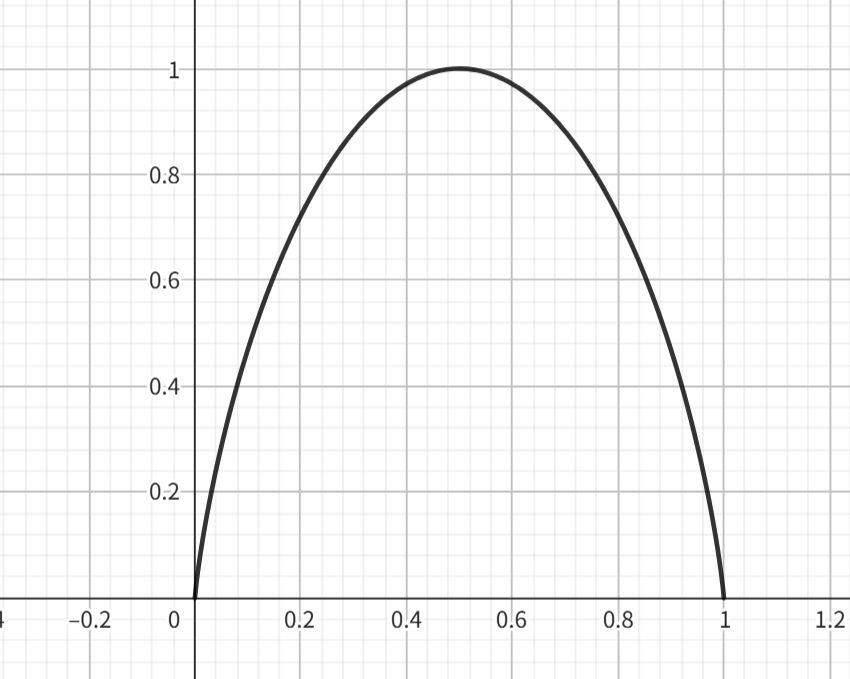
\includegraphics[width=.6\textwidth]{images/c2_1.png}
    \caption{$H=x\log 1/x + (1-x)\log 1/(1-x)$的图像}
\end{figure}
\chapter{Lecture 3}

%--- 信息 ----
\begin{center}
    讲师:王立威 \qquad
    课程时间:25.Mar.4th \qquad 
    笔记:25.June.7th
\end{center}

\bigskip

考虑一般的$p$进制编码(经典比特为$p=2$进制,但也有3进制计算机)此时,随机元$X$的熵为 
\[
H(X) := \sum_{i=1}^n p_i \log_p 1/p_i
\]
相应地,这个量的单位也应该从bit变为其他的单位. 

上节课说到均匀分布时熵最大,可以总结成如下命题
\begin{proposition}
    对于$X = (m_1, \dots, m_n)$,那么$H(X) \le \log_2 n$
\end{proposition}
\begin{proof}
    使用Jensen不等式即可,此略.
\end{proof}

事实上,熵的定义非常符合直觉,我们通过一个例子感受 
\begin{example}
    我们考虑随机变量$X,Y,Z$. $X$有分布列$(p_1,\dots, p_n)$,其中$p_n = q_1 + q_2$;$Y$的分布列正比于$(q_1, q_2)$;$Z$有分布列$p_1,\dots, p_{n-1}, q_1, q_2$. 

    可以写成如下形式:
    \[
    \begin{matrix}
        X: & p_1 & p_2 & \cdots & p_n(= & q_1 + q_2) \\
        Y: & \ & \ & \ & \dfrac{q_1}{q_1 + q_2} & \dfrac{q_2}{q_1 + q_2}  \\
        Z: & p_1 & p_2 & \cdots & q_1 & q_2
    \end{matrix}
    \]

    此时$H(X),H(Y),H(Z)$满足什么关系?
\end{example}
\begin{solution}
    应该满足$H(X) + p_n\cdot H(Y) = H(Z)$,下面通过计算来说明.
    \begin{align*}
        & H(Z) - H(X) \\
        = & \ \left[
            \sum_{i=1}^{n-1} p_i \log_2 1/p_i + \sum_{j=1}^2 q_j \log_2 1/q_j
        \right] - \left[
            \sum_{i=1}^{n-1} p_i \log_2 1/p_i + 
            p_n \log_2 1/p_n
        \right] \\
        = & \ \sum_{j=1}^2 q_j \left(
            \log 1/q_j - \log_2 1/p_n
        \right) \\
        = & \ \sum_{j=1}^2 q_j \log_2\dfrac{q_1 + q_2}{q_j} \\
        = & \ p_n \sum_{j=1}^2 \dfrac{q_j}{q_1 + q_2} \log_2\dfrac{q_1 + q_2}{q_j} = p_n \cdot H(Y)
    \end{align*}

    通过上面的例子,我们发现熵的定义十分合理.$Y$可以视作对于$X$在$m^{(X)}_n$的情况下的进一步阐释(细化);而$Z$直接融合了$X$和$Y$对其的阐释.阐释发生的概率是$p_n$,所以$Z$的信息量就是$X$的信息量加上$p_n$倍$Y$的信息量.
\end{solution} 

以上结论对于$\boldsymbol{q}$是更高维的情况下也成立,称作\textbf{熵的加性}. 

我们至此讨论了熵的定义和性质,但回归到实际实践当中,我们当然需要$l_i$全部为整数.换言之,对于随机变量$X$服从分布列$P=(p_1,\dots, p_n)$,我们想要构造一个具体的编码算法,得到平均码长最短的实际编码$C = (c_1, \dots, c_n)$,称\textbf{最优码}. 以下,我们记$c_i$的长度为$\abs{c_i}$

可以得到最优码的一些性质:
\begin{itemize}
    \item 如果$p_1 \ge p_2 \ge \cdots \ge p_n$,那么对于最优码一定有$\abs{c_1} \le \abs{c_2} \le \cdots \le \abs{c_n}$ 
    \item Kraft不等式取等条件成立: $\sum_{i=1}^n 2^{-\abs{c_i}} = 1$ 
    \item 如果$p_1 \ge p_2 \ge \cdots \ge p_n$,那么会有$\abs{c_n} = \abs{c_{n-1}}$. (直观而言,这是在说二叉树中$c_n$一定会有兄弟;数学而言,这是为了满足上一条性质的等号要求)
    \item 若$(c_1, \dots, c_n)$是$(p_1,\dots, p_n)$的最优码,那么$(c_1, \dots, \tilde{c}_{n-1})$是$(p_1,\dots, p_{n-1}+p_n)$的最优码.其中我们假定$c_{n-1}, c_n$在二叉树中是兄弟,仅有最后一位不同,而$\tilde{c}_{n-1}$代表它们二者前面的公共前缀.(该性质可通过反证法得出)
\end{itemize}

结合这些性质便可以设计算法,逐步将问题的维度降低.这个算法就是Huffman编码(自行查阅该算法,此不介绍). 

接下来拓展一下熵的定义,对于多个变量可定义联合熵. 
\begin{definition}[联合熵]
    对于两个随机变量$X,Y$,联合分布列为$P_{X,Y} = (p_{i,j})$,定义\textbf{联合熵}(joint entropy)为 
    \[
    H(X, Y) := \sum_{i,j} p_{i,j} \log_2 1/p_{i,j}
    \]
\end{definition}

可见这样的定义和原本熵的定义很类似,意义是将$X,Y$一起编码时的最短平均码长;$X,Y$一共的信息量等等. 

\begin{theorem}
    对于两个随机变量$X,Y$,有$H(X,Y) \le H(X) + H(Y)$,取等当且仅当$X,Y$独立.
\end{theorem}

\begin{example}
    取$X=Y$,可以发现$H(X, Y) = H(X) \le 2H(X) = H(X) + H(Y)$
\end{example}

类似地,可以定义条件熵
\begin{definition}[条件熵]
    对于两个随机变量$X,Y$,对于$X$的可能取值$x_i$(满足$\Pr[X = x_i] > 0$),定义 
    \[
H(Y|X=x_i) := \sum_{j} \Pr[Y=y_j | X = x_i] \log_2 \dfrac{1}{\Pr[Y=y_j | X = x_i]}
    \]

    总体的\textbf{条件熵}(conditional entropy)就定义为 
    \[
H(Y|X) := \sum_{i} \Pr[X = x_i] H(Y|X=x_i)
    \]
\end{definition} 

以下定理说明条件熵$H(Y|X)$的意义为“$Y$在$X$的基础上引入的新信息”:
\begin{theorem}
    对于两个随机变量$X,Y$,有 
    \[
    H(X,Y) = H(X) + H(Y|X) = H(Y) + H(X|Y)
    \]
\end{theorem}

% \begin{figure}[H]
%     \centering
%     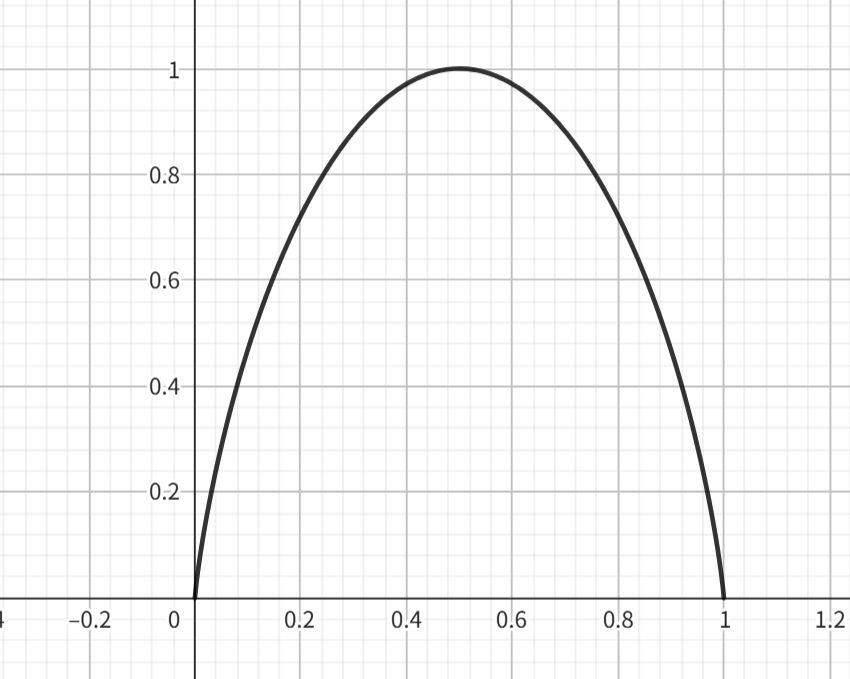
\includegraphics[width=.6\textwidth]{images/c2_1.png}
%     \caption{$H=x\log 1/x + (1-x)\log 1/(1-x)$的图像}
% \end{figure}
\chapter{Lecture 4}

%--- 信息 ----
\begin{center}
    讲师:王立威 \qquad
    课程时间:25.Mar.11th \qquad 
    笔记:25.June.7th
\end{center}

\bigskip

接着上节课的内容,根据上节课的两个定理可以得到:
\[
H(Y) \ge H(Y|X), \qquad H(X) \ge H(X|Y)
\]

这说明原有的信息量永远不小于条件下的信息量.这称作"Conditioning reduces entropy.",可以认为这是因为加上条件等价于在某种程度上引入了信息,从而降低了“新”的信息量. 

事实上,我们能推出 
\[
H(X) - H(X|Y) = H(Y) - H(Y|X) = H(X) + H(Y) - H(X,Y)
\]

据此引出新的定义 
\begin{definition}[互信息]
    对于两个随机变量$X,Y$,定义其\textbf{互信息}(mutual information)为 
    \[
    I(X;Y) := H(X) - H(X|Y) = H(X) + H(Y) - H(X,Y)
    \]
\end{definition}

互信息是可以用联合概率分布列表示的,表示法如下(请自行验证):
\[
I(X; Y) = \sum_{i,j} \Pr[X=x_i, Y=y_j] \log_2 \dfrac{\Pr[X=x_i, Y=y_j]}{\Pr[X=x_i]\cdot \Pr[ Y=y_j]}
\]

自然地,可类似定义任意多元随机变量$\boldsymbol{X}=(X_i)_{i=1}^n$的联合熵$H(\boldsymbol{X})$;也可定义两组随机变量$\boldsymbol{X}=(X_i)_{i=1}^n, \boldsymbol{Y}=(Y_j)_{j=1}^m$的条件熵$H(\boldsymbol{X}|\boldsymbol{Y})$和互信息$I(\boldsymbol{X};\boldsymbol{Y})$. 

\begin{theorem}
    对于多元随机变量$\boldsymbol{X}=(X_i)_{i=1}^n$,有 
    \[
    H(\boldsymbol{X}) = H(X_1) + H(X_2|X_1) + H(X_3|X_1,X_2) + \cdots + H(X_n|X_{1\sim (n-1)})
    \]
\end{theorem}

至此的讨论都基于随机变量$X$的分布列$P$是已知的,但在真实世界中我们往往无法精确观测或获取真实分布列.但取而代之,我们往往有一个估计(近似)$Q = (q_1,\dots, q_n)$,此时我们依照这个分布列编码,码长应为$(\log 1/q_1,\dots, \log 1/q_n)$,那么平均码长为 $\sum_{i=1}^n p_i \log 1/q_i$. 相较与最短码长$H(P)$,这样的编码存在冗余$\sum_{i=1}^n p_i \log p_i/q_i$,这就是著名的K-L散度. 

\begin{definition}[Kullback-Leibler 散度]
    对于两个分布列$P=(p_1,\dots, p_n)$和$Q=(q_1,\dots, q_n)$,其\textbf{Kullback-Leibler 散度}(divergence)定义为 
    \[
    D(P \| Q) := \sum_{i=1}^n p_i \log_2 \dfrac{p_i}{q_i}
    \]

    Kullback-Leibler 散度也称作K-L散度或相对熵(relative entropy).并且也可记作$\text{KL}(P\| Q)$.
\end{definition}

某种意义而言,K-L散度是比信息熵更加基础和重要的概念.在以后的例子中,我们会发现在有些情况下难以定义信息熵,但却可以定义K-L散度. 

另外,请注意K-L散度不是对称的,故不是距离度量.

\begin{example}[K-L散度的凸性]
    考虑以下情况:固定$Q$,$D$对$P$是凸的吗?固定$P$,$D$对$Q$是凸的吗?$D$对$(P, Q)$是凸的吗?
\end{example} 
\begin{solution}
    事实上,K-L散度是凸的.
\end{solution}

除了K-L散度,我们还有别的定义分布列距离的方式,一个比较经典的是全变分距离(1-范数)
\begin{definition}[全变分距离]
    对于两个分布列$P=(p_1,\dots, p_n)$和$Q=(q_1,\dots, q_n)$,其\textbf{全变分距离}(total variance)定义为 
    \[
    \norm{P-Q}_1 := \sum_{i=1}^n \abs{p_i - q_1}
    \]
\end{definition}

KL-散度和全变分距离之间有如下关系:
\begin{theorem}[Pinsker不等式]
    对于两个分布列$P, Q$,有 
    \[
    \norm{P - Q}_1 \le \sqrt{2\ln 2\cdot D(P \| Q)}
    \]
\end{theorem}
\begin{proof}
    首先我们对最简单的Bernoulli分布形式进行验证.  也就是设$P=(p, 1-p), Q = (q, 1-q)$,此时通过暴力计算可以验证Pinsker不等式.  

    对于一般情况的$P,Q$,我们定义:
    \[
    \tilde{P} = \left(
        \sum_{i:p_i \ge q_i} p_i, 
        \sum_{i:p_i < q_i} p_i
    \right), \quad 
    \tilde{Q} = \left(
        \sum_{i:p_i \ge q_i} q_i, 
        \sum_{i:p_i < q_i} q_i 
    \right)
    \]

    不难验证$\norm{P - Q}_1 = \norm{\tilde{P} - \tilde{Q}}_1$. 而另一方面,根据K-L散度的凸性可以知道$D(\tilde{P} \| \tilde{Q}) \le D(P \| Q) $

    而$\tilde{P}, \tilde{Q}$都是Bernoulli分布,我们通过先前的计算已经获知其满足Pinsker不等式,于是 
    \[
    \norm{P - Q}_1 = \norm{\tilde{P} - \tilde{Q}}_1 \le \sqrt{2 \ln 2\cdot D(\tilde{P} \| \tilde{Q})} \le \sqrt{2 \ln 2\cdot D(P \| Q)}
    \]

    至此证毕. 
\end{proof}

% \begin{figure}[H]
%     \centering
%     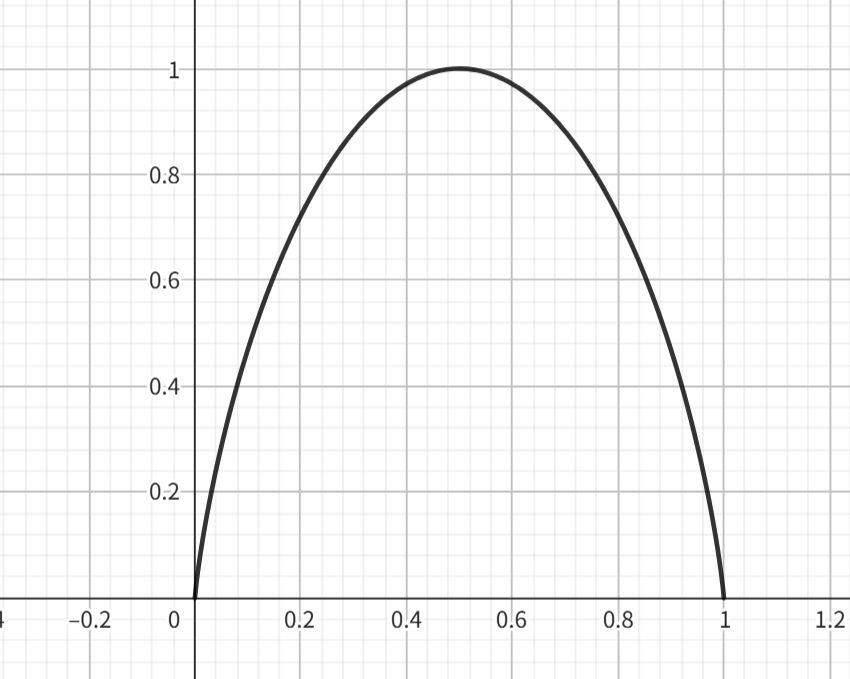
\includegraphics[width=.6\textwidth]{images/c2_1.png}
%     \caption{$H=x\log 1/x + (1-x)\log 1/(1-x)$的图像}
% \end{figure}
\chapter{Lecture 5}

%--- 信息 ----
\begin{center}
    讲师:王立威 \qquad
    课程时间:25.Mar.18th \qquad 
    笔记:25.June.7th
\end{center}

\bigskip

首先讨论了Pinsker不等式的证明方法,我直接放在了上一章当中. 

接下来看新的内容.  我们先来看一个例子来深入理解最短编码和信息熵之间的差距. 也就是要求整数和不要求整数之间的差距.  
\begin{example}
随机变量$X$,分布列$P=(0.01, 0.99)$ 
\begin{itemize}
    \item 信息熵$H(X) \approx 0.07 $\text{bit}.
    \item 最短编码1 bit.
\end{itemize}
\end{example}

事实上,我们有如下推论 
\begin{corollary}
    对于任意随机变量$X$,最短编码和信息熵的差严格小于1.
\end{corollary}

因此,通过差值来衡量编码效率是不合适的,我们应该使用比值来衡量.  另一方面,我们设定要传输可列次信息,也就是说存在一个i.i.d的序列$X_1, X_2,\dots$和$X$同分布.  我们传输这些信息时,不妨每$T$个打包成一组进行传输,可见这样一次传输的平均最小码长$l_{\min}$满足 
\[
l_{\min}(X_1, \dots, X_T) \le H(X_1, \dots, H_T) + 1 = T\cdot H(X) + 1
\] 

于是比值 
\[
\text{Ratio} = \dfrac{l_{\min}(X_1, \dots, X_T)}{H(X_1, \dots, H_T)} \le 1 + \dfrac{1}{T \cdot H(X)} = 1 + O\left(\dfrac{1}{T} \right)
\]

平均到编码每一个信息所需的长度有上界$\frac{T H(X) + 1}{T} \ra H(X)$.  因此,在$T \ra \infty$时,最终的平均码长应该趋于$H(X)$,而非$l_{\min}(X)$.  这也是为什么我们认为信息熵是一个本质的定义.  

值得指出,这样的操作在实际实践中会带来更大的时延. 

上面的模型其实对实际情况做了一个简化,也就是假设每个时刻的信息都是i.i.d的. 为了泛化我们的模型,我们应该将信源建模成随机过程(stochastic process)$\mathcal{X} = (X_t)_{t\ge 1}$,下面讨论这个模型.  

首先需要定义这个信源的平均码长. 
\begin{definition}[熵率]
    对于随机信源$\mathcal{X} = (X_t)_{t\ge 1}$,定义其\textbf{熵率}(entropy rate)为 
    \[
    H(\mathcal{X}):= \lim_{T \ra \infty} \dfrac 1T \cdot H(X_1, X_2, \dots, H_T)
    \]

    我们假定上述极限存在(这个技术细节过于琐碎,略去)
\end{definition}

另一种角度而言,我们也可以认为$H(\mathcal{X})$是每个时刻增加的新的信息. 
\begin{theorem}
    给定信源$\mathcal{X}= (X_t)_{t\ge 1}$,假设以下极限存在,那么下式成立. 
    \[
    H(\mathcal{X}) = \lim_{T \ra \infty} H(X_T | X_1, X_2, \dots, H_{T-1})
    \]
\end{theorem}
\begin{proof}
    注意到
    \[
    H(X_1, X_2, \dots, H_T) = H(X_1) + \sum_{i=2}^T H(X_i | X_{1 \sim (i-1)})
    \]

    使用数学分析(I)中的结论便可完成证明. 
\end{proof} 

接下来考虑连续随机变量的编码,但显然它没有所谓“最短平均码长”这一概念,我们只能先形式上给出一个熵的定义:
\begin{definition}[微分熵]
    对于连续型随机变量$X$,设其p.d.f.为$f(x)$,则定义其\textbf{微分熵}(differential entropy)为 
    \[
        h(X) := -\int_{\R} f(x) \log_2 f(x) \dx
    \]
\end{definition}

这个形式上定义并非单纯的望文生义,而是真正的有本之木!我们考虑连续型随机变量$X$对应的离散化版本$X_\Delta$,其中$\Delta > 0$是一个离散化的粒度. 具体而言,$X_\Delta$只取值于$k\Delta, \ (k \in \Z)$,并且 
\[
\Pr[X_\Delta = k\Delta] = \Pr[k \Delta \le X < (k+1)\Delta] = \int_{k \Delta }^{(k+1) \Delta} f(x) \dx
\]

可以得到如下的近似 
\begin{proposition}
    对于连续型随机变量$X$对应的离散化版本$X_\Delta$,有 
    \[
    h(X) + \log \dfrac{1}{\Delta} \approx H(X_\Delta)
    \]
\end{proposition}

另外,微分熵和香农熵在性质上也有一些不同的地方. 我们知道对于离散随机变量$X$,
\begin{itemize}
    \item 若$Y = X + c$,则$H(X) = H(Y)$
    \item 若$Z = aX (a>0)$,则$H(X) = H(Z)$
\end{itemize}

但对于连续随机变量和微分熵,对应的结论会变为
\begin{proposition}
    对于连续型随机变量$X$,若$Y = X + c$(其中$c$是常数),那么
    \[
    h(Y) = h(X)
    \]
\end{proposition}
\begin{proposition}
    对于连续型随机变量$X$,若$Z = aX$(其中$a>0$是常数),那么
    \[
    h(Z) = h(X) + \log a
    \]
\end{proposition}

下面举隅一例来计算其微分熵.
\begin{example}
    已知随机变量$X \sim \mathcal{N}(\mu, \sigma^2)$,求$h(X)$.
\end{example}
\begin{solution}
    我们记$X$的概率密度函数为$f(x)$,有 
\[
f(x) = \dfrac{1}{\sigma \sqrt{2\pi}} \exp\left\{
    -\dfrac{(x - \mu)^2}{2 \sigma^2}
    \right\}
\]
 
因此, 
\begin{align*}
    h(X) & = -\int_{-\infty}^{\infty} f(x) \log_2 f(x) \dx \\
    & = -\int_{-\infty}^{\infty} f(x) \cdot \left(
        -\log_2(\sigma \sqrt{2\pi}) - \dfrac{(x - \mu)^2}{2 \ln 2\cdot \sigma^2}
    \right) \dx \\
    & = \log_2(\sigma \sqrt{2\pi}) \int_{-\infty}^{\infty} f(x)\dx + \dfrac{1}{2 \ln 2\cdot \sigma^2} \int_{-\infty}^{\infty} (x-\mu)^2 f(x)\dx \\
    & = \log_2(\sigma \sqrt{2\pi}) + \dfrac{1}{2 \ln 2\cdot \sigma^2} \var(X) \\
    & = \log_2(\sigma \sqrt{2\pi}) + \dfrac{1}{2 \ln 2} \\ 
    & = \dfrac{1 + \log_2(\pi e \sigma^2)}{2}
\end{align*}

至此便得到了答案.
\end{solution}

% \begin{figure}[H]
%     \centering
%     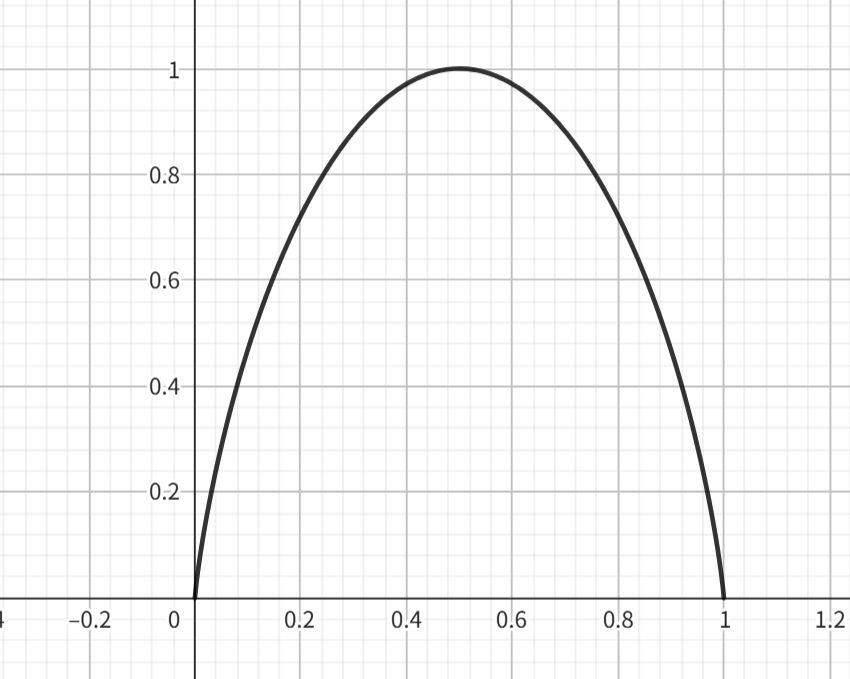
\includegraphics[width=.6\textwidth]{images/c2_1.png}
%     \caption{$H=x\log 1/x + (1-x)\log 1/(1-x)$的图像}
% \end{figure}
\chapter{Lecture 6}

%--- 信息 ----
\begin{center}
    讲师:王立威 \qquad
    课程时间:25.Mar.25th \qquad 
    笔记:25.June.7th
\end{center}

\bigskip

接着将之前对于离散型随机变量定义的各种熵迁移到连续型随机变量上来 
\begin{definition}[联合微分熵]
    对于两个连续型随机变量$X,Y$,设其联合p.d.f.为$f_{X,Y}(x,y)$,定义其\textbf{联合微分熵}(joint differential entropy)为 
    \[
    h(X, Y) := - \int\int f_{X,Y}(x, y) \log f_{X,Y}(x, y) \dx\dx[y]
    \]
\end{definition}
\begin{definition}[条件微分熵]
    对于两个连续型随机变量$X,Y$,设其联合p.d.f.为$f_{X,Y}(x,y)$,定义其\textbf{条件微分熵}(conditional differential entropy)为 
    \[
    h(X| Y) := - \int\int f_{X,Y}(x, y) \log f_{X|Y}(x, y) \dx\dx[y]
    \]
\end{definition}

下面来讨论一个很重要的量:互信息。 
\begin{definition}[连续型随机变量的互信息]
    对于两个连续型随机变量$X, Y$,具有概率密度$f_{X,Y}, f_{X|Y}, f_{Y|X}$等,定义它们的\textbf{互信息}(mutual information)为 
    \[
    I(X; Y):= h(X) - h(X|Y)
    \]
\end{definition}

这样从形式上定义的互信息竟然保留了离散版本的诸多性质!
\begin{theorem}
    对于两个连续型随机变量$X, Y$,一定有
    \[
    I(X;Y) = h(Y) - h(Y|X) = h(X) + h(Y) - h(X, Y)
    \]

    另外,还可以用联合概率密度和边缘概率密度来表达
    \[
    I(X; Y) = \int\int f_{X,Y}(x, y) \log \dfrac{f_{X,Y}(x,y)}{f_X(x) f_Y(y)} \dx\dx[y]
    \]
\end{theorem}

为什么会造成这样的性质呢?我们考虑它们二者的对应的离散化版本$X_\Delta, Y_\Delta$,会有 
\[
I(X; Y) = \lim_{\Delta\ra 0^+} I(X_\Delta, Y_\Delta)
\]

这说明虽然在连续意义下,微分熵的物理意义不是非常明确,但互信息的物理意义是充分明晰的。

另外,也可以接着定义K-L散度(相对熵)
\begin{definition}
    给定$f,g$分别是连续型随机变量$X,Y$的概率密度函数,定义\textbf{K-L散度}为 
    \[
    \text{KL}(f\| g) := \int f(x) \log \dfrac{f(x)}{g(x)} \dx
    \]
\end{definition}

继续考虑离散化版本$X_\Delta, Y_\Delta$以及他们对应的分布列$P_\Delta, Q_\Delta$。可以发现 
\[
\lim_{\Delta \ra 0^+} \text{KL}(P_\Delta \| Q_\Delta) = \text{KL}(f\| g)
\]

至此,关于信源编码就告一段落了。

现在考虑编码的问题,对于一个随机对象,希望知道最小的描述长度。但这个问题是不平凡的,因为就算是退化到了确定对象也难以严格定义“描述长度”。 好比对于圆,我们可以使用圆心和半径;对于矩形可以使用中心、长和宽;但对于一个比较混沌的图形就难以描述了。

\begin{figure}[H]
    \centering
    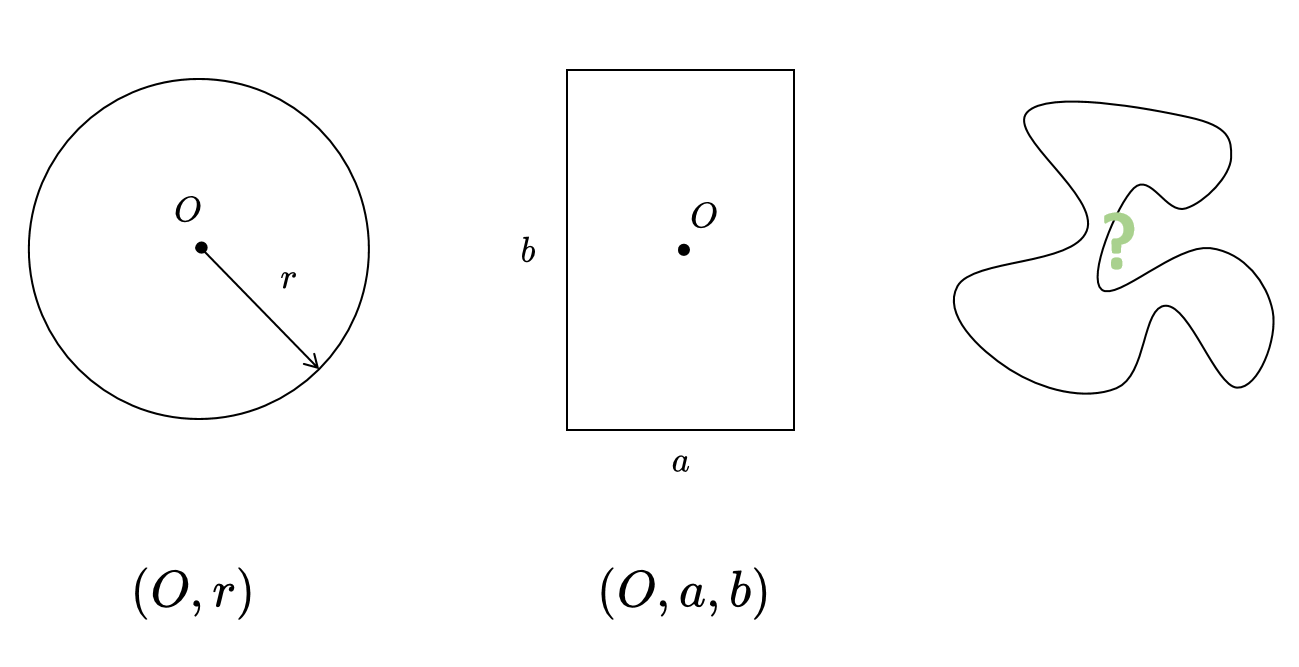
\includegraphics[width=.75\textwidth]{images/c6_1.png}
\end{figure}

这个所谓的“对象”空间太大了,需要限制一下范围,并挖掘本质。 前苏联的数学家Kolmogorov给出了回答,将其限制在了字符串$\{0,1\}^*$当中。

\begin{example}
    直觉上,可以将$000\cdots 0$描述成$n$个0;将$011011011\cdots$描述成$m$个011;但如果原字符串很混乱,那最好的描述不过是将其复述一遍。
\end{example}

这样的直觉需要转为严谨的定义,思考一下就会发现我们需要发掘“计算”的本质。这个问题Turing已经回答了,是“Turing机”(如今的Boole线路与这个模型也是等价的)。那么所有问题都一定有解吗?并不是,证明也很简单。 

\begin{theorem}
    我们考虑所有的决定问题,即给定集合$L \sbe \{0, 1\}^*$,需要对任意的$x\in \{0,1\}^*$判断$x$是否属于$L$。 一定存在某个$L_0$对应的决定问题不存在Turing机上可以解决该问题的算法。
\end{theorem}
\begin{proof}
    记所有的问题构成的集合基数为$\kappa$,记所有算法构成的集合基数为$\lambda$。 对于Turing机,算法本质上就是一个字符串,所以$\lambda$是$\{0, 1\}^*$的基数。而上面的讨论说明了一个$L$可以决定一个问题,故$\kappa$是$\mathcal{P}(\{0, 1\}^*)$的基数。 

    根据Cantor定理,有 
    \[
    \lambda = \card {\{0, 1\}}^* < \card \mathcal{P} \Big( {\{0, 1\}}^* \Big) = \kappa
    \]

    基数不同,所以不存在双射。 因此一定存在一个不可解的问题。
\end{proof}

我们可以讲出这样的不可计算问题,例如说“停机问题”。可以证明:给定算法$A$和输入$i$,不存在算法保证一定可以计算$A$是否可以在有限步内停下。 

Turing的工作其实在一定程度上收到了Godel的启发,在Turing关于计算本质问题的研究工作发表前,Godel证明了任意一阶逻辑的不完备性,也正是熟知的“Godel不完备定理”.
\chapter{Lecture 7}

%--- 信息 ----
\begin{center}
    讲师:王立威 \qquad
    课程时间:25.Apr.1st \qquad 
    笔记:25.June.8th
\end{center}

\bigskip

接着上一课程未解决的问题,我们如何定义一个确定对象的“最短描述长度”。此前,我们已经将这个对象的范围缩小到$x \in \{0,1\}^*$,加上Turing给出的计算模型,我们已经具备定义Kolmogorov复杂度的能力了!(关于下面用到的通用Turing机(universal Turing machine)这一概念,请自行浏览资料)
\begin{definition}[Kolmogorov复杂度]
    对于一个字符串$x \in \{0,1\}^*$,其对于一个通用Turing机$U$的\textbf{Kolmogorov复杂度}(complexity)定义为 
\[
K_U(x) := \min_{p, U(p)=x} \abs{p}
\]

也就是$U$要决定$x$所需的最短“代码”长度,这也简称为K-复杂度,并简写为$K(x)$.
\end{definition}

若没有学过Turing机相关的知识,可以暂时理解成$U$是某个固定的编程语言,例如C++或Python等。以下命题说明了上面将$U$简写是合理的:
\begin{proposition}
    设$U, U'$是两个通用Turing机,那么存在一个常数$c \in \N$使得对于任意$x \in \{0, 1\}^*$,如下不等式成立 
    \[
    K_U(x) \le K_{U'}(x) + c
    \]

    其中$c$只依赖于$U,U'$而不依赖于$x$.
\end{proposition}

但这个定义听起来很难实践。一种尝试计算$x$的K-复杂度的方式,是从根据长度小到大遍历所有的$p$(由于$K_U(x)$一定存在有界,所以需要遍历的$p$是有限多的),但这会遇到一个难题:“停机问题”。我们无法判断对于特定的$p$,$U$是否会停机。 归根结底,这是因为$K_U$本质上是不可以计算的!
\begin{theorem}
    $K_U(x)$是不可计算的. 
\end{theorem}
\begin{proof}
    这里只给出大致的思想,UTM的细节略去。假设存在一个算法$P_0$,可以对于任意$x$计算$K_U(x)$. 

    记$\abs{P_0} = l$,下面给出一个新的算法$P_0'$。首先我们将$\{0,1\}^*$中的元素排序成$s_1,s_2,\dots,s_i,\dots$。
    
    $P_0'$如下:
    \begin{itemize}
        \item 令变量$i$遍历$1,2,\dots$
        \begin{itemize}
            \item 使用$P_0$计算$K_U(s_i)$
            \item 若$K_U(s_i) \ge L$,则输出$s_i$
        \end{itemize}
    \end{itemize}

    那么可见$\abs{P_0'} = l + c$($c$常数). 而$P_0'$可以决定识别字符串$s$,其中$K_U(s) \ge L$。但根据K-复杂度的定义,会有 
    \[
    L \le K_U(s) \le \abs{P_0'} = l + c
    \]

    所以取$L$充分大便可得到矛盾. 因此$K_U$不可计算.
\end{proof}

关于这部分告一段落,我们来看概率分布估计的问题,也就是说对于一些函数$g_i$,已知$\E_X\sim P [g_i(X)]$的值,求原始分布$P$。 这类问题往往具有无穷多个解,我们应当关心其中某个具有优良性质的。 
    \begin{definition}[最大熵估计]
        给定一族函数$\{g_i(x)\}_{i\in I}$和$\{r_i\}_{i \in I}$。\textbf{最大熵估计}指的是如下问题的解 
        
        \begin{align*}
            \maximize_{f} \ & -\int f(x) \ln f(x) \dx \\
            \text{s.t.} \ & \int f(x) \dx = 1 \\
            \ & \int g_i(x)f(x) \dx = r_i\quad ,i\in I
        \end{align*}
    \end{definition}

这里将所谓“熵”从$\log_2$替换成$\ln$是因为他们只差一个倍数。 我们试着求解一个最大熵问题:
\begin{example}
    给定一个连续型随机变量$X$及其p.d.f. $f(x)$,已知
    \[
    \E[X] = 0, \qquad \var(X) = \sigma^2
    \]
    
    求最大熵分布. 
\end{example}
\begin{solution}
    一般而言,这类问题的通法时使用Lagrange乘子和变分。不过这里我们可以给出一个使用K-L散度的解法。 


\end{solution}
% \begin{figure}[H]
%     \centering
%     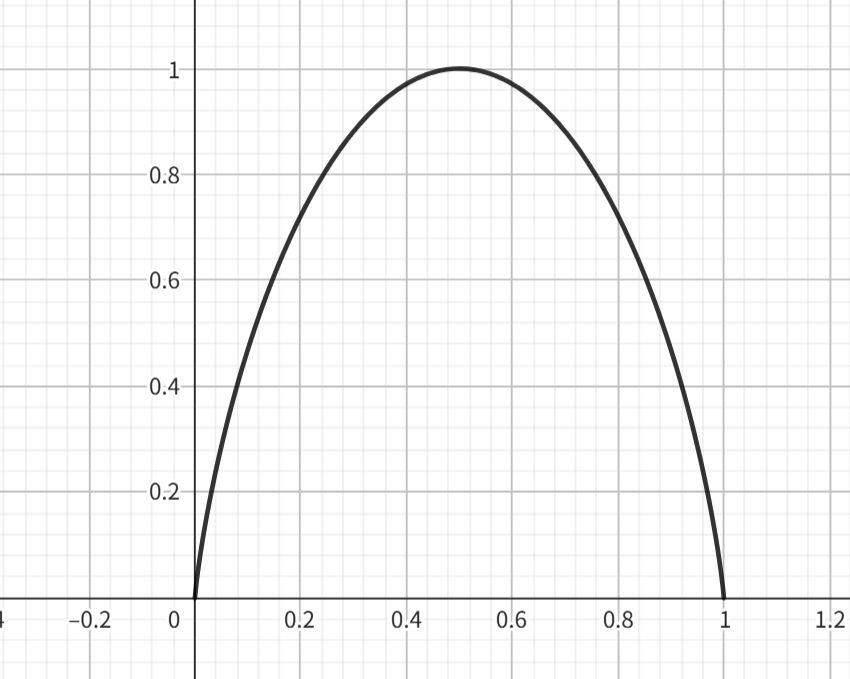
\includegraphics[width=.6\textwidth]{images/c2_1.png}
%     \caption{$H=x\log 1/x + (1-x)\log 1/(1-x)$的图像}
% \end{figure}
\chapter{Lecture 8}

%--- 信息 ----
\begin{center}
    讲师:王立威 \qquad
    课程时间:25.Apr.8th \qquad 
    笔记:25.June.8th
\end{center}

\bigskip

来讨论信道编码,动机在于真实世界的信道都是含噪的,噪声会干扰信息的传递致使接收到的信息和发送的信息不完全相同. 自然地,我们想要设计一套算法来纠正由噪声引起的错误,这套算法应该包含编码(encoding)和解码(decoding)两部分. 

\begin{example}
    一个最简单的想法就是编码时重复三次,解码时取众数. 
\end{example}

上面的例子虽然简单,但却内蕴了深刻的思想——解码时将内容映射到最近邻的合理码字. 这里的最近邻使用的是Hamming距离(请自行查阅). 

我们设$M_i$对应的编码是$c_i$(对于所有$1 \le i \le n$),那么有如下定理:
\begin{theorem}
    对于正整数$t > 0$,若对于任意$i\neq j$都有$d_H(c_i,c_j) \ge 2t + 1$,那么这样的编码可以纠正$t$比特的错误. 
\end{theorem}

我现在希望将信息空间映射到编码空间 
\[
\text{Message Space} \quad \{0,1\}^m \quad \quad \longrightarrow \quad \quad
\text{Coding Space} \quad \{0,1\}^n 
\]

现在给定$t,m$,来估计一下$n$的下界. 
\begin{proposition}
    上述条件下,需要满足 
    \[
    2^n \ge 2^m \cdot {\sum_{i=1}^t \binom{n}{i}}
    \]
\end{proposition}
\begin{proof}
统计一下球形邻域$B(x):= \{y:d_H(x,y) \le t\}$的大小,注意到对于任意$i\neq j$,要有$B(c_i)\cap B(c_j) = \varnothing$
\end{proof}

接着来计算其上界. 这里我们将目标重述为给定$m$和$ \de \in (0, 1/2)$,找一个尽量小的$n$使得一定存在编码$c_1, c_2, \dots, c_{2^m} \in \{0,1\}^n$使得
\[
d_H(c_i, c_j) \ge \de n , \quad \forall i \neq j
\]

采用概率方法(这是现代组合数学的常用技巧)可以证明如下结论. 
\begin{theorem}[Gilbert-Vashamov界]
    如果对于某个常数$c$($c$依赖于$\de$),$n \ge cm$,那么存在一组编码符合条件.
\end{theorem}
\begin{proof}
    我们在$\{0,1\}^n$上独立且均匀地采样$c_1, c_2, \dots, c_n$,相当于每个比特都服从均匀两点分布. 故$d_H(c_i,c_j) \sim B(n, 1/2)$.  根据Chernoff Bound,可以得到 
\[
\Pr \Big[
d_H(c_i, c_j) < \de n  
\Big] < e^{- \ln 2  D(\de \| 1/2) \cdot n} = e^{-O(n)}
\]

根据Union Bound,又有 
\[
\Pr \left[
    \bigcup_{i,j \in [2^m]: i\neq j} d_H(c_i, c_j) < \de n
\right] < \binom{2^m}{2}e^{-O(n)}
\]

所以 
\[
\Pr \Big[
    \forall i\neq j \in [2^m],\ d_H(c_i,c_j) \ge \de n
\Big] \ge 1 - \binom{2^m}{2}e^{-O(n)}
\]

我们只需要上式右侧大于0即可,化简可以得到这需要 
\[
n \ge \Omega(m)
\]

也就证明了结论. 事实上,这个$c$可以取成$\dfrac{2}{D(\de \| \frac 12)}$. 
\end{proof}

总结一下设计一套纠错码的流程:
\begin{enumerate}
    \item 首先要设计一组码字$c_1,c_2,\dots, c_N$,使得它们彼此Hamming距离充分大(达到预期纠错的能力). 
    \item 然后给出一个编码算法,将消息映射到码字. 
    \item 最后给出解码算法,找到接受消息最近的码字. 
\end{enumerate}

这里的第3步比较特殊,一般$m$可以来到上百的量级,码字计算会来到2的上百次方量级,朴素寻找最近邻码字是不现实的. 我们必须要考虑编码和解码的计算复杂度.  这部分也是该领域着重努力的方向.  

一个最早期的做法是Hamming码,在介绍Hamming码之前,先通过一个例子感受一下. 在陈述例子之前,我们先定义零空间. 
\begin{definition}
    对于域$F$上的线性映射$T: U \ra V$,定义其\textbf{零空间}(null space)为
    \[
    \Null (T):= \{x\in U: Tx = 0\}
    \]

    如果$T$有矩阵表示$A$,那么也称为矩阵的零空间$\Null (A)$. 
\end{definition}
\begin{example}
    考虑$GF(2)$上的矩阵 
    \[
    H = \begin{bmatrix}
        0 & 0 & 0 & 1 & 1 & 1 & 1 \\ 
        0 & 1 & 1 & 0 & 0 & 1 & 1 \\ 
        1 & 0 & 1 & 0 & 1 & 0 & 1 \\ 
    \end{bmatrix}_{3 \times 7}
    \]

    试计算 $\min\limits_{x,y \in \Null(H): x\neq y} d_H(x,y)$.
\end{example}

我们用列向量表示矩阵$H = \begin{bmatrix}
    v_1, & v_2, & \cdots & ,v_7
\end{bmatrix}$. 可以看出$v_i$事实上就是$i$的二进制表示. 可以看出这个7个向量张成的空间是3维的. 

不难验证$\Null(H)$事实上是$[2]^7$的一个线性子空间. 而$d_H(x, y)$其实是$x + y$为1的比特数,也就是1-范数. (这里$+$是$GF(2)$中的运算符)这里我们称$\norm{x}_1$为$x$的\textbf{权重}. 而若
\[
Hx = \sum_{i=1}^7 v_i x_i = 0
\]

结合之前关于维度的讨论可知$\norm{x}_1 \ge 3$,所以$d_H(x,y) \ge 3$. 另一方面取
\[
x = \begin{bmatrix}
    0 & 0 & 0 & 0 & 0 & 0 & 0
\end{bmatrix}^\top, \quad 
y = \begin{bmatrix}
    1 & 1 & 1 & 0 & 0 & 0 & 0
\end{bmatrix}^\top
\]

可以达到下界,故答案就是$3$. 

% \begin{figure}[H]
%     \centering
%     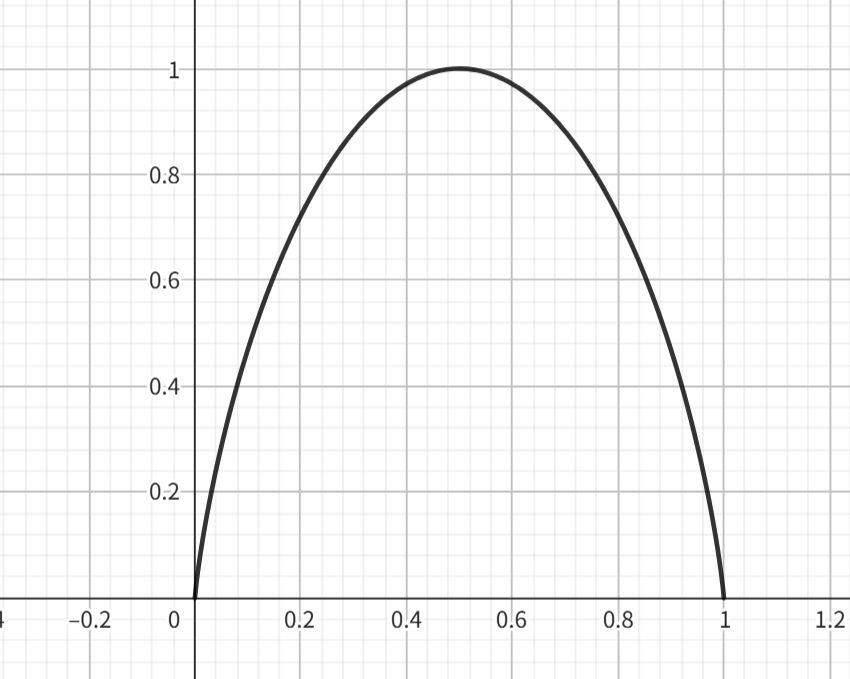
\includegraphics[width=.6\textwidth]{images/c2_1.png}
%     \caption{$H=x\log 1/x + (1-x)\log 1/(1-x)$的图像}
% \end{figure}
\chapter{Lecture }

%--- 信息 ----
\begin{center}
    讲师:王立威 \qquad
    课程时间:25. \qquad 
    笔记:\today
\end{center}

\bigskip

% \begin{figure}[H]
%     \centering
%     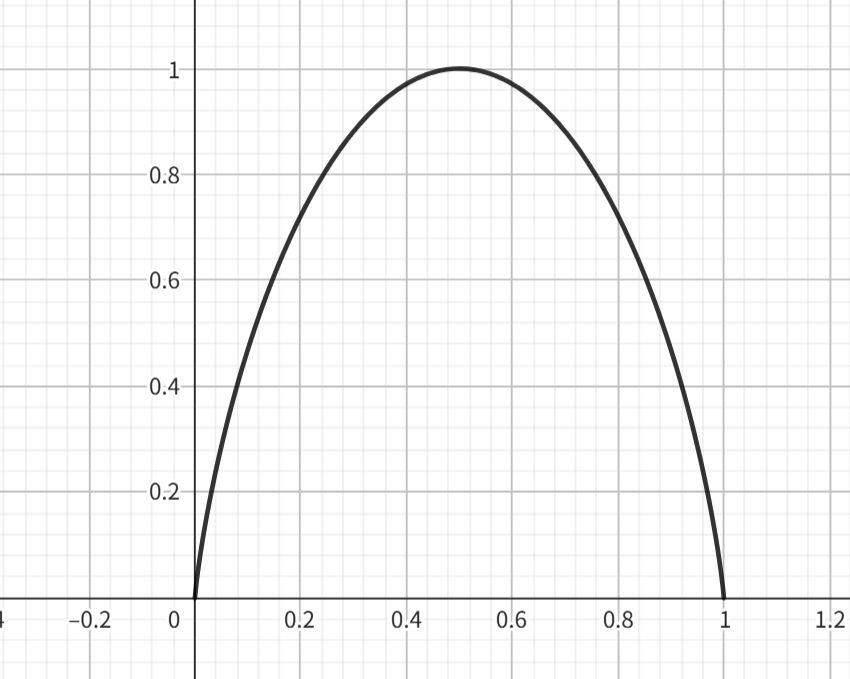
\includegraphics[width=.6\textwidth]{images/c2_1.png}
%     \caption{$H=x\log 1/x + (1-x)\log 1/(1-x)$的图像}
% \end{figure}
\chapter{Lecture }

%--- 信息 ----
\begin{center}
    讲师:王立威 \qquad
    课程时间:25. \qquad 
    笔记:\today
\end{center}

\bigskip

% \begin{figure}[H]
%     \centering
%     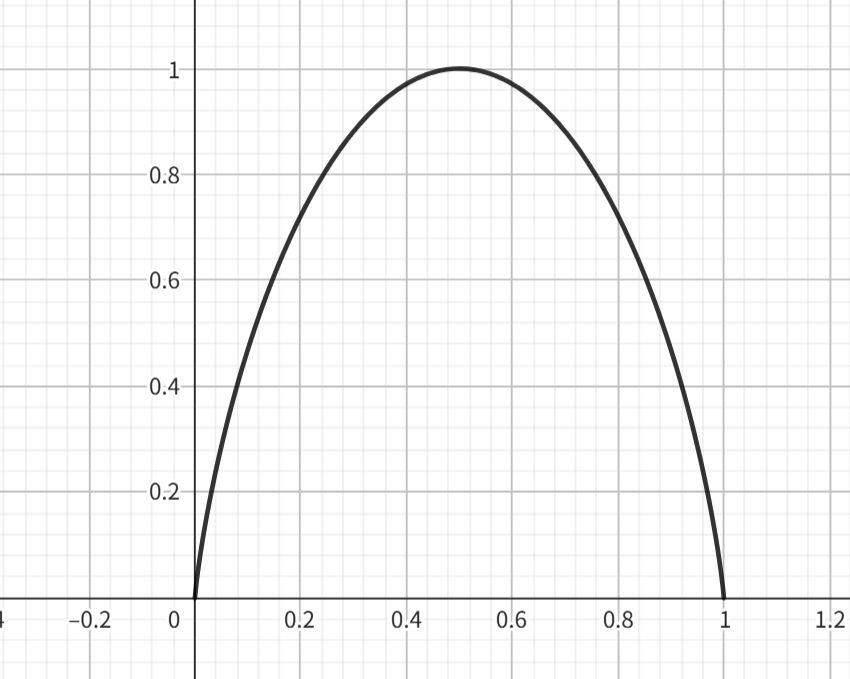
\includegraphics[width=.6\textwidth]{images/c2_1.png}
%     \caption{$H=x\log 1/x + (1-x)\log 1/(1-x)$的图像}
% \end{figure}
\chapter{Lecture }

%--- 信息 ----
\begin{center}
    讲师:王立威 \qquad
    课程时间:25. \qquad 
    笔记:\today
\end{center}

\bigskip

% \begin{figure}[H]
%     \centering
%     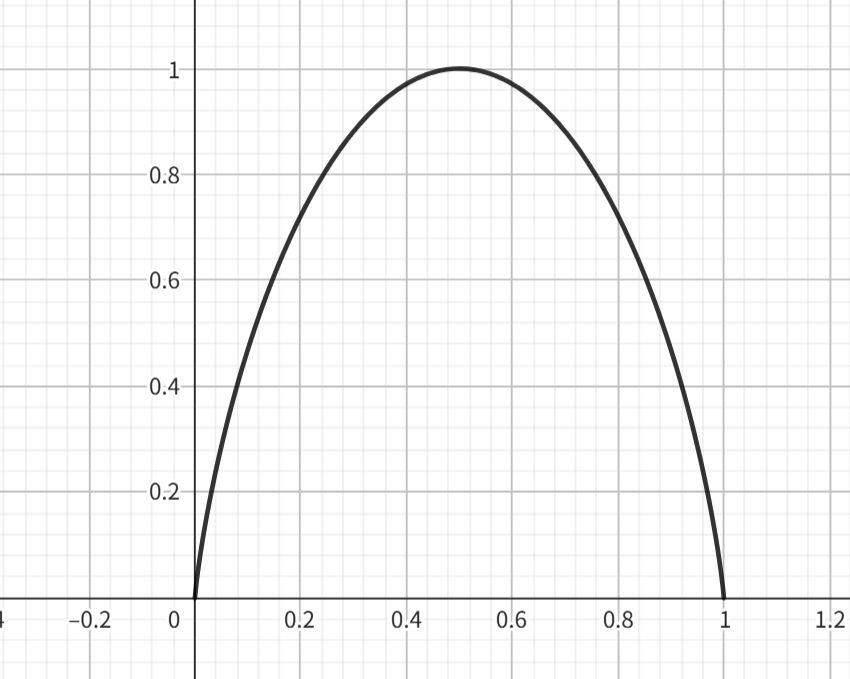
\includegraphics[width=.6\textwidth]{images/c2_1.png}
%     \caption{$H=x\log 1/x + (1-x)\log 1/(1-x)$的图像}
% \end{figure}
\chapter{Lecture }

%--- 信息 ----
\begin{center}
    讲师:王立威 \qquad
    课程时间:25. \qquad 
    笔记:\today
\end{center}

\bigskip

% \begin{figure}[H]
%     \centering
%     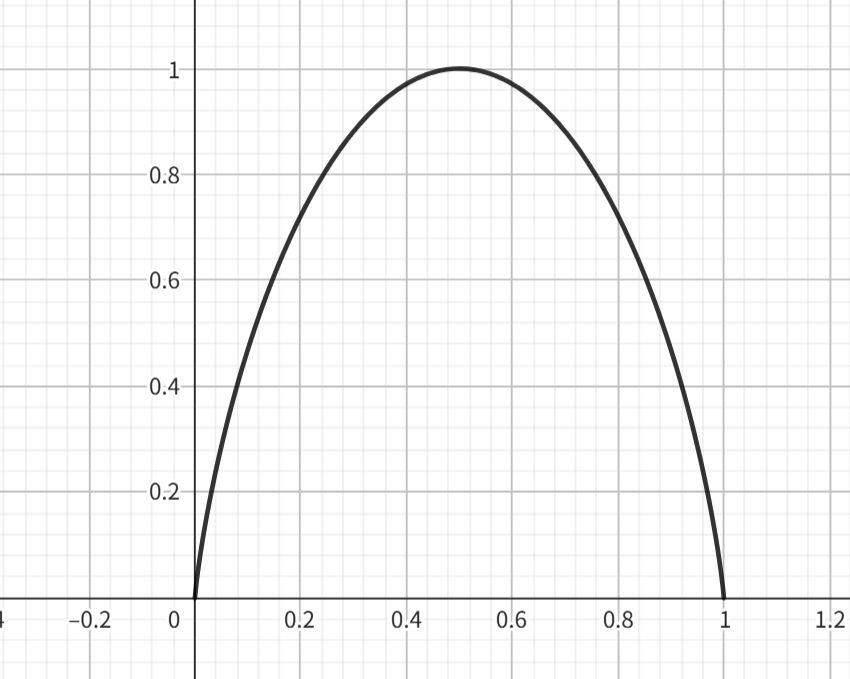
\includegraphics[width=.6\textwidth]{images/c2_1.png}
%     \caption{$H=x\log 1/x + (1-x)\log 1/(1-x)$的图像}
% \end{figure}
\chapter{Lecture 13}

%--- 信息 ----
\begin{center}
    讲师:王立威 \qquad
    课程时间:25.May.20th \qquad 
    笔记:25.June.9th
\end{center}

\bigskip

首先完成了信道编码定理的证明,放在了前一节. 下面介绍Fisher信息和Carm​​ér-Rao不等式. 

动机和来源是无偏估计. (若学过统计学可跳过)
\begin{definition}[无偏估计]
    我们(往往独立同分布地)采样了一组样本点$X=(X_1,X_2,\dots, X_n)$,设其密度函数为$f(\cdot;\te)$(其中$\te$是我们要估计的参数),那么有 
    \[
    f(x;\te) = \prod_{i=1}^n f(X_i; \te)
    \]
    
    现在使用这些样本点得到$\te$的一个估计$\hat{\te} = \phi(X_1,\dots, X_n)$. 如果满足$\E[\hat{\te}] = \te$则称$\hat{\te}$是$\te$的\textbf{无偏估计}(unbiased estimation).
\end{definition} 

在正式定义Fisher信息之前先要引入得分函数的定义. 
\begin{definition}[得分函数]
    \textbf{得分函数}(score function)是指 
    \[
    S(X;\te) := \del{}{\te} \ln f(X;\te)
    \]
\end{definition}

\begin{proposition}
    得分函数满足$\E[S(X;\te)] = 0$
\end{proposition}
\begin{proof}
    根据定义 
    \begin{align*}
        \E[S(X;\te)] & = \int S(x;\te) f(x;\te) \dx \\
        & = \int \del{}{\te} \ln f(x;\te) f(x;\te) \\
        & = \int \del{f(x;\te)}{\te} \dfrac{1}{f(x;\te)} f(x;\te) \dx \\ 
        & = \int \del{f(x;\te)}{\te} \dx \\
        & = \del{}{\te}\int f(x;\te) \dx = \del{}{\te} \ 1 = 0
    \end{align*}
\end{proof} 

现在可以定义Fisher信息了
\begin{definition}[Fisher信息]
    对于$X,\te$,定义其Fisher信息(information)为 
    \[
    I(\te) := \var(S(X;\te)) = \E[S^2(X;\te)]
    \]
\end{definition}

\begin{proposition}
    $I(\te) = -\E\left[
        \del{^2}{\te^2} \ln f(X;\te)
    \right] = -\displaystyle\int \del{^2}{\te^2} \ln f(x;\te) f(x;\te) \dx$
\end{proposition}
\begin{proof}
    \begin{align*}
       \E\left[
        \del{^2}{\te^2} \ln f(X;\te)
    \right] & =\int \del{^2}{\te^2} \ln f(x;\te) f(x;\te) \dx \\
    & = \int \del{}{\te} \left(
        \dfrac{\nabla_\te f(x;\te)}{f(x;\te)}
    \right) f(x;\te) \dx \\
    & = \int \dfrac{\nabla^2_\te f(x;\te)\cdot f(x;\te) - (\nabla_\te f(x;\te))^2}{f^2(x;\te)} f(x;\te) \dx \\
    & = \int \nabla^2_\te f(x;\te) \dx - \int \left(\dfrac{\nabla_\te f(x;\te)}{f(x;\te)}\right)^2 f(x;\te) \dx \\
    & = \del{^2}{\te^2} \int f(x;\te) \dx -\int \del{^2}{\te^2} \ln f(x;\te) f(x;\te) \dx \\
    & = -\E\left[
        \del{^2}{\te^2} \ln f(X;\te)
    \right]
    \end{align*}
\end{proof} 

Fisher信息的意义在衡量无偏估计最好能好到什么程度,这里的好是由方差来度量的. 也就是这里要介绍的不等式:
\begin{theorem}[Cram​​ér-Rao不等式]
    对于任意$\te$的无偏估计$\phi: X \ra \R$,我们有 
    \[
    \var(\phi(X)) \ge \dfrac{1}{I(\te)}
    \]
\end{theorem}
\begin{proof}
    证明此略.
\end{proof}

我们可以将得分函数,Fisher信息,Cramér-Rao不等式拓展到$d$维的情况:

\begin{align*}
    \del{}{\te} \ln f(X;\te) \quad & \longrightarrow \quad \nabla_\te \ln f(x;\te) \\ 
    -\E\left[
        \del{^2}{\te^2} \ln f(X;\te)
    \right]\quad & \longrightarrow \quad -\E\left[
        \nabla^2_\te \ln f(X;\te)
    \right] \\
    \var(\phi(X)) \ge \dfrac{1}{I(\te)} \quad & \longrightarrow \quad  \cov(\phi(X)) \ge \dfrac{1}{I(\te)}
\end{align*}

% \begin{figure}[H]
%     \centering
%     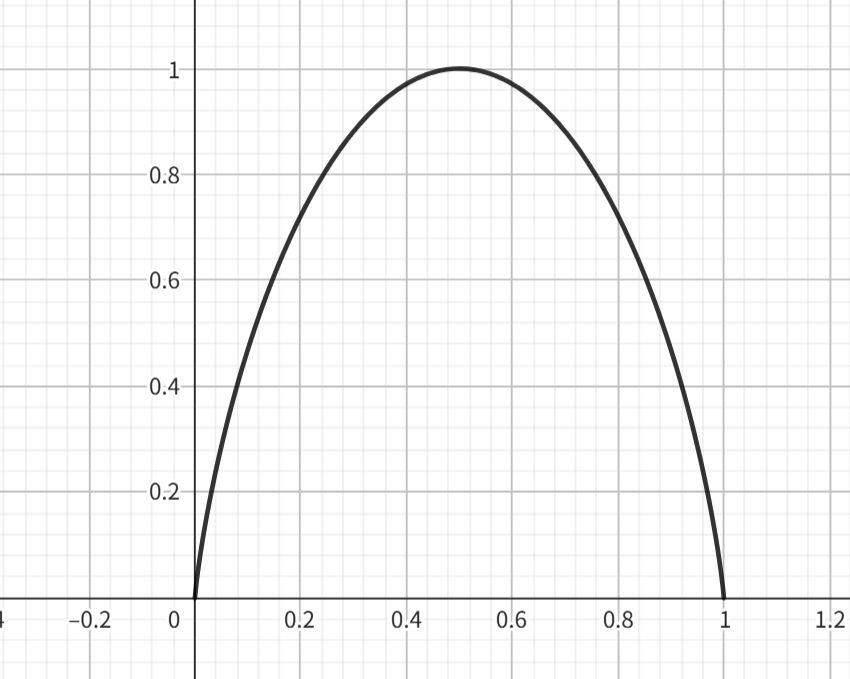
\includegraphics[width=.6\textwidth]{images/c2_1.png}
%     \caption{$H=x\log 1/x + (1-x)\log 1/(1-x)$的图像}
% \end{figure}
\chapter{Lecture }

%--- 信息 ----
\begin{center}
    讲师:王立威 \qquad
    课程时间:25. \qquad 
    笔记:\today
\end{center}

\bigskip

% \begin{figure}[H]
%     \centering
%     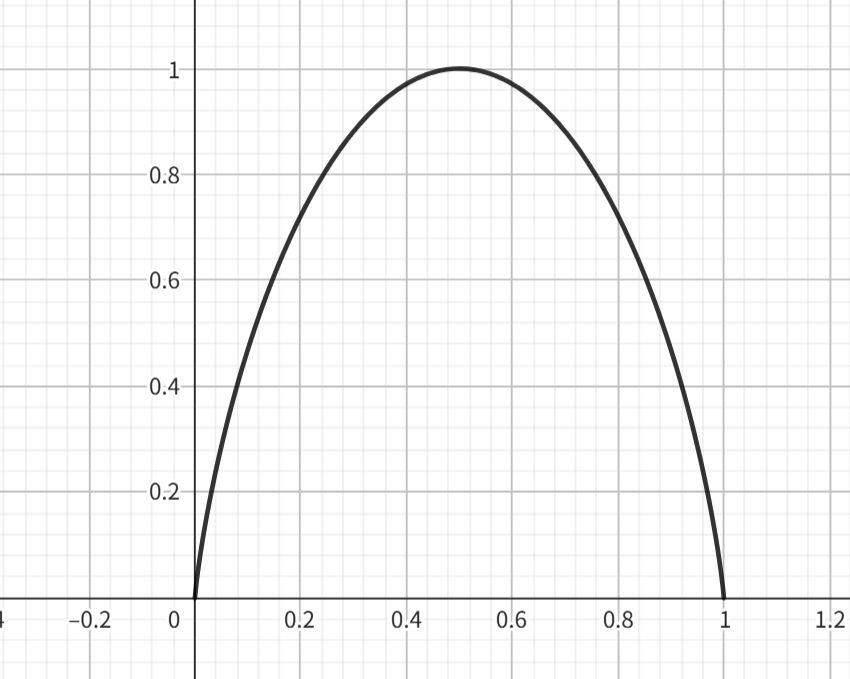
\includegraphics[width=.6\textwidth]{images/c2_1.png}
%     \caption{$H=x\log 1/x + (1-x)\log 1/(1-x)$的图像}
% \end{figure}
\chapter{Lecture }

%--- 信息 ----
\begin{center}
    讲师:王立威 \qquad
    课程时间:25. \qquad 
    笔记:\today
\end{center}

\bigskip

% \begin{figure}[H]
%     \centering
%     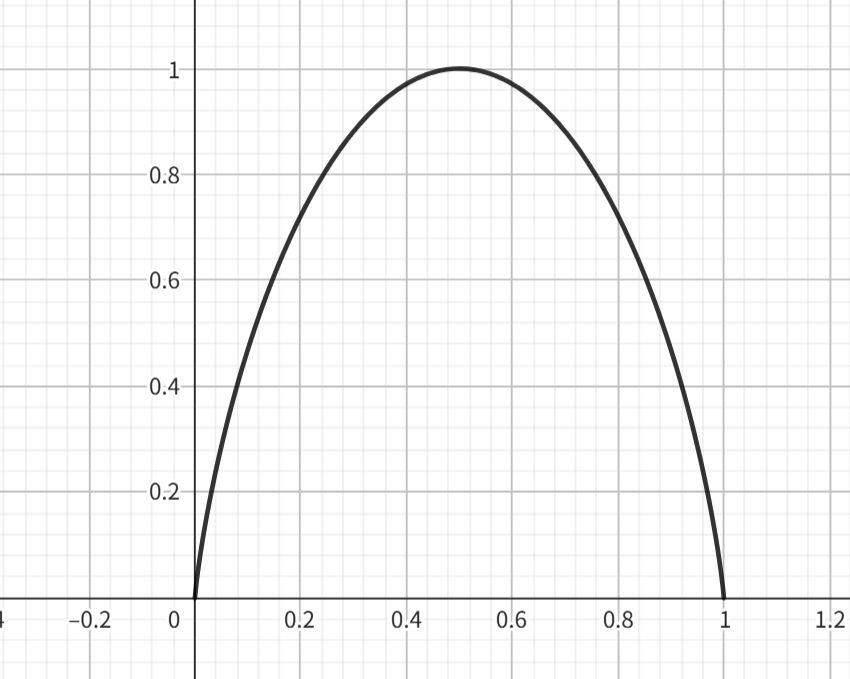
\includegraphics[width=.6\textwidth]{images/c2_1.png}
%     \caption{$H=x\log 1/x + (1-x)\log 1/(1-x)$的图像}
% \end{figure}

\end{document}